\section{Las im�genes de piel y sus caracter�sticas}

Las im�genes con las que trabajamos son fotograf�as en bruto, sin ning�n tipo de tratamiento previo, tomadas con c�maras de mano, lo que hace que la calidad de las mismas sea muy variable. Dichas fotograf�as no fueron tomadas para realizar nuestro trabajo, sino que forman parte de la base de datos de im�genes de la Universidad de Iowa, publicadas en la p�gina http: //hardinmd.lib.uiowa.edu/DERMPICTURES.HTML. En esta base hallamos fotograf�as de muy variada calidad. Uno de los principales problemas con los que nos topamos al momento de analizarlas, fue la diferencia en la iluminaci�n de las im�genes, lo que causa zonas de luz y oscuridad muy marcadas. No fue un tema menor la escala utilizada en cada una de las im�genes, por tal motivo debimos considerar que la distancia del observador a las ampollas puede ser muy variable. Para que el m�todo presentado detecte de manera exitosa las ves�culas, uno de los requisitos que se debi� tener presente al momento de seleccionar las fotograf�as es que la escala de la imagen muestre la ves�cula en primer plano. Como por ejemplo, en las im�genes de la figura \ref{fig:imagenOk2}. En tanto que, la ves�culas presentes en las im�genes de la figura \ref{fig:imagenesEscalaInutilizable} mayormente no fueron localizadas, dado que dichas fotografias fueron tomadas a una distancia mayor. Este tipo de im�genes fueron descartadas del subconjunto con el cual trabajamos.

\begin{figure}[ht]
\centering
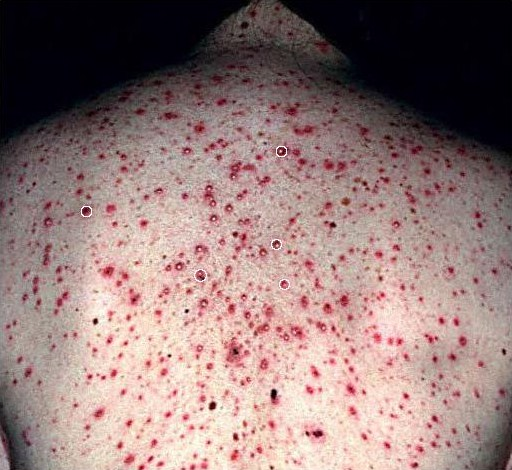
\includegraphics[scale=0.25]{Resources/resultado-chicken_pox_picture_01.jpg}
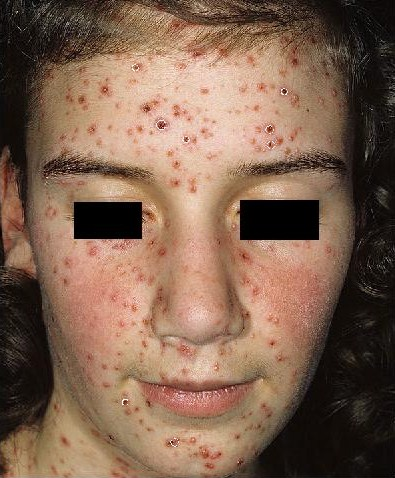
\includegraphics[scale=0.25]{Resources/resultado-varicella_9.jpg}
\caption{Ejemplos de im�genes no utilizables debido a su escala \label{fig:imagenesEscalaInutilizable}}
\end{figure}

Generalmente las ves�culas de varicela se presentan con una forma circular, pero existen excepciones, con lo cu�l debimos tener presente que no siempre la detecci�n de c�rculos ser�a apropiada para detectar la ves�cula. Cuando nos centramos en analizar el color de las ves�culas de varicela, nos encontramos con la presencia de colores un tanto alejados del color real de la ves�cula, debido a la calidad de las fotograf�as. Esto dificult� el an�lisis de las mismas. Por �ltimo, debimos tener en cuenta el ruido que presentan las im�genes que utilizamos, esto puede ser desde lunares, pelos e irregularidades propias de la piel y hasta inscripciones agregadas en las fotograf�as e incluso la calidad de las mismas. Dadas estas particularidades de las im�genes utilizadas, debimos extraer un subconjunto de im�genes homog�neo, que nos permitiera aplicarles m�todos generales para las detecciones de forma y color.

\begin{figure} [ht]
\centering
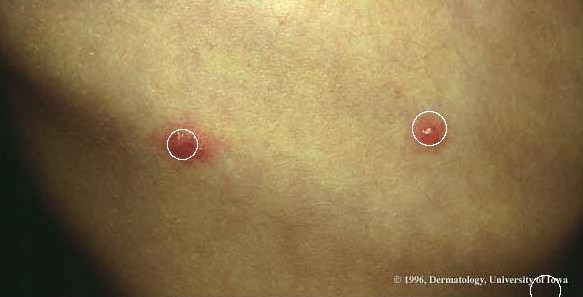
\includegraphics[scale=0.25]{Resources/resultado-Varicel-03.jpg}
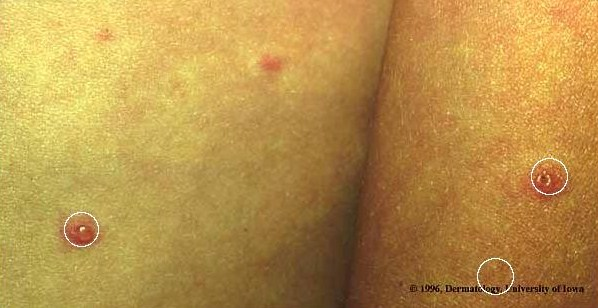
\includegraphics[scale=0.24]{Resources/resultado-Varicel-04.jpg}
\caption{Ejemplos de im�genes con una escala tal que es posible detectar las ves�culas \label{fig:imagenOk2}}
\end{figure}
